\documentclass[a4paper, 12pt]{article}

% Pacchetti utili
\usepackage[utf8]{inputenc}
\usepackage[T1]{fontenc}
\usepackage[italian]{babel}
\usepackage{graphicx}
\usepackage{hyperref}
\usepackage{geometry}
\usepackage{enumitem}
\geometry{margin=2.5cm}
\usepackage{titlesec}
\renewcommand\thesubsection{\thesection.\alph{subsection}}
\usepackage{amsmath}

% Titolo e autore
\title{
    Documentazione del Progetto FantaSanremo \\
    \large Basi di Dati
}

\author{
    \textbf{GRUPPO 46} \\
    \vspace{1em}
    {\small
    Luca Ciardullo S5798102,
    Giulio Rossi S6413167,
    Gabriele Traversa S6072517.
    }
}


\date{\today}

\begin{document}

\maketitle
\tableofcontents
\newpage

% ============================
\section{Requisiti Disambiguati}
% Inserisci qui tutte le assunzioni fatte sul dominio e ogni chiarimento rispetto alla specifica dei requisiti originale.
Le informazioni da salvare per un utente, prese dal sito ufficiale di FantaSanremo sono:
\begin{itemize}
    \item \textbf{Username} (univoco);
    \item \textbf{Email} (univoca);
    \item \textbf{Password} (ad esempio hashed, ma ne ignoriamo l'implementazione sicura);
    \item \textbf{Consenso} (al trattamento dei dati).
\end{itemize}

\noindent Per ogni UTENTE, SQUADRA, LEGA, ARTISTA e BONUS possiamo salvare un'immagine che lo rappresenta, in quanto sono presenti sul sito ufficiale FantaSanremo (non è obbligatorio che sia presente un'immagine per ogni istanza).
\newline Esiste una sola lega \textit{MONDIALE}, ogni utente parteciperà automaticamente al momento della creazione del proprio account e non avrà possibilità di uscirne.
\newline Ogni SQUADRA parteciperà automaticamente alla lega mondiale al momento della creazione e non ci sarà possibilità di rimuoverla
\newpage
\section{Progetto Concettuale}


\subsection{Schema ER}
% Inserisci lo schema ER (come immagine o codice TikZ).
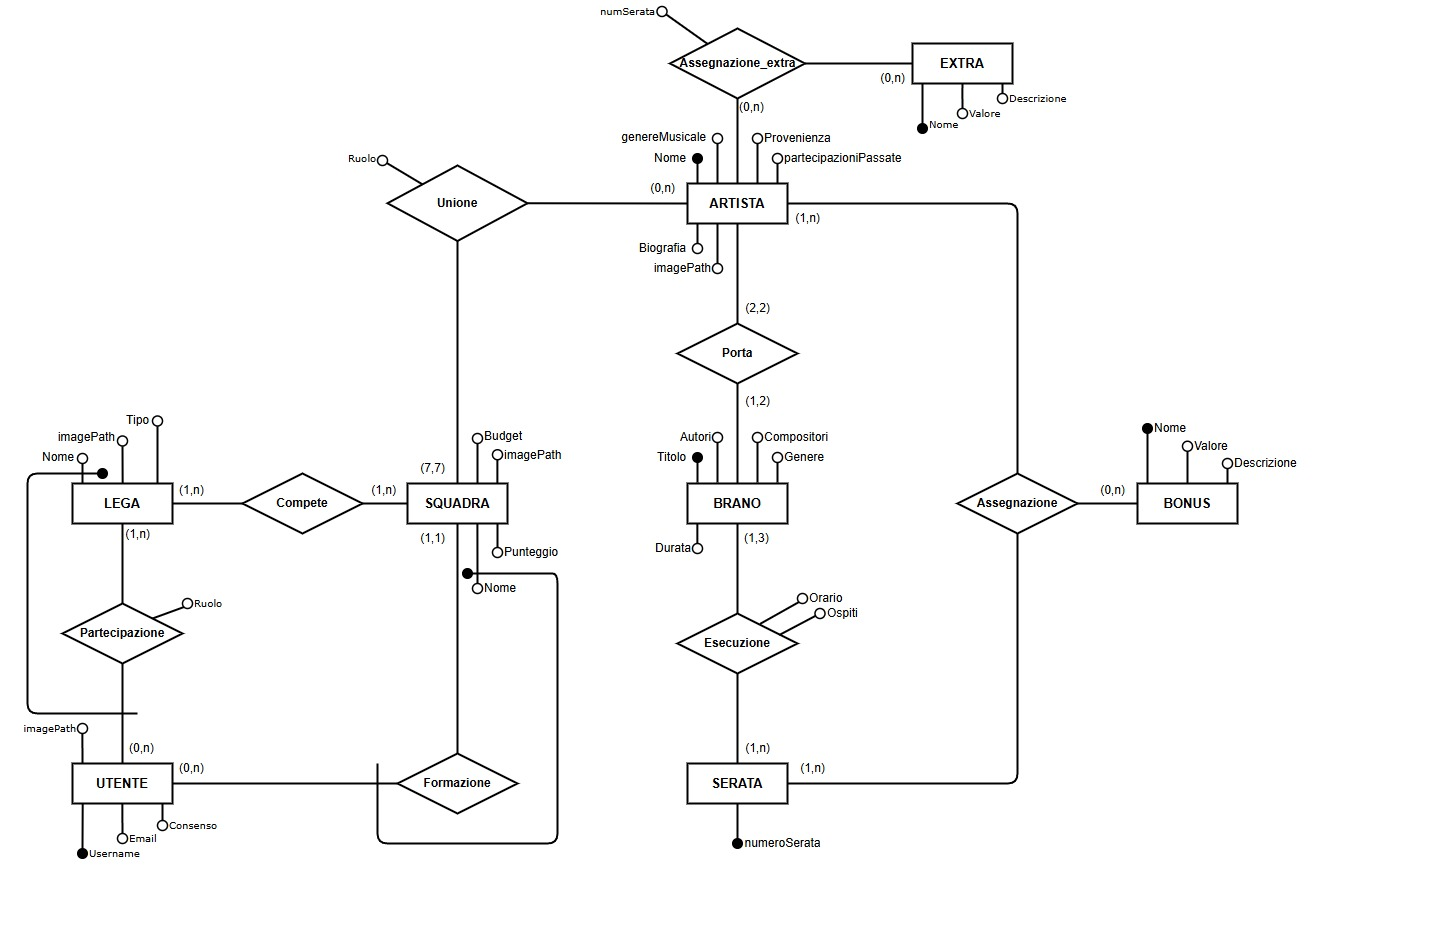
\includegraphics[width=\textwidth]{er-schema.jpeg}

\subsection{Dizionario Dati e Domini Attributi}
% Inserisci qui la tabella con i domini degli attributi e la descrizione delle entità.

\[
\begin{array}{ll}
\text{dom}(ruolo, \text{Unione}) = \text {array di 5 elementi con dom = } \\ 
    \{ \text{CAPITANO}, \text{TITOLARE}, \text{RISERVA}, \text{UNKNOWN} \} \\
\text{dom}(tipo, \text{LEGA}) = \{ \text{PUBBLICA}, \text{PRIVATA}, \text{SEGRETA}, \text{MONDIALE} \} \\
\text{dom}(nome, \text{SERATA}) = \{ \text{PRIMA}, \text{SECONDA}, \text{TERZA}, \text{COVER}, \text{FINALE} \} \\
\text{dom}(serata, \text{Assegnazione}) = \{ \text{PRIMA}, \text{SECONDA}, \text{TERZA}, \text{COVER}, \text{FINALE} \} \\
\text{dom}(consenso, \text{UTENTE}) = \text{BOOL (corrisponde al consenso al trattamento dei dati specificato} \\
\text{dall'utente, viene richiesto durante l'iscrizione al FantaSanremo, può essere modificato)}
\end{array}
\]

Gli attributi \textit{imagePath} sono stringhe con l'url di un'immagine specifica memorizzata (assumiamo) nel nostro sistema, se è vuota allora non è presente alcuna immagine, per esempio: \\
- UTENTE.imagePath è l'url dell'immagine di profilo dell'utente \newline
- BONUS.imagePath è l'url dell'immagine dell'eventuale sponsor di tale bonus; l'imagePath del BONUS \textit{Bold} avrà l'url all'immagine dello sponsor MOTOROLA, mentre per il BONUS \textit{Ballerini} avrà stringa vuota in quanto bonus senza sponsor. \newline
(Queste immagini sono facilmente visibili sul sito ufficiale FantaSanremo)

\subsection{Vincoli}
SQUADRA.budget sarà un intero con default (e massimo) 100 al momento della creazione della squadra, decrementato e incrementato durante la modifica della squadra, e utilizzato principalmente per non effettuare nuovamente ad ogni singola operazione il calcolo dei baudi rimanenti.

Per ogni SQUADRA, e per ogni SERATA i ruoli devono essere così spartiti:
1 Capitano, 4 Titolari e 2 Riserve,
i ruoli per la serata successiva possono essere cambiati durante la settimana del Festival ogni giorno da mercoledì 12 febbraio a sabato 15 febbraio dalle 08.00 alle 20.00,
i ruoli sono salvati in un array di serate per tenere traccia dei ruoli per ogni serata (sarà necessario per avere lo storico dei bonus assegnati).
Se l'utente non effettua modifiche entro l'orario di scadenza, verranno mantenute le scelte del giorno prima.
% Elenca e descrivi tutti i vincoli concettuali che non sono rappresentabili nel diagramma ER (cardinalità, condizioni, ecc.)

\subsection{Gerarchie di Generalizzazione}
Nessuna Gerarchia di Generalizzazione utilizzata.
% Specifica le generalizzazioni usate e il tipo (totale/parziale, disgiunta/sovrapposta).

\subsection{Modifiche Apportate e Risposte a Segnalazioni}

- abbiamo modificato l'attributo "nome" di "LEGA" e "SQUADRA" perché abbiamo notato che possono esistere più leghe e squadre con lo stesso nome ma create da utenti diversi, tra "LEGA" e "UTENTE" abbiamo dovuto aggiungere una nuova associazione chiamata "Crea".

- abbiamo modificato l'attributo "ruolo" dell'associazione "Partecipa" tra "LEGA" e "UTENTE" con un booleano per indicare se è o meno amministratore.

- abbiamo corretto la cardinalità dell'associazione tra "ARTISTA" e "BRANO" (1,2) di "ARTISTA" in (2,2) perché è obbligato PERFORZAAAA, e non puoi farci niente, a portare due brani il suo e quello della serata cover e (1,1) di "BRANO" in (1,2) perché , come visto in questo festival, due artisti possono gareggiare assieme nella serata cover con lo stesso brano.

- abbiamo aggiunto l'attributo "serata" nell'associazione "Assegnazione" per indicare la serata in cui è stato assegnato il bonus all'artista così da raddoppiarlo in caso di capitano.

- abbiamo cambiato i nomi dell'entità "BONUS" in "BONUS-SERALI", perché abbiamo notato che solo quella perticolare categoria di bonus vengono ripetuti in ogni serata, e "EXTRA" in "BONUS" perché tutti i bonus sono singoli per artista e non possono essere riottenuti in più serate.

- abbiamo aggiunto l'attributo "extra" alla nuova entità "BONUS" per indicare i bonus extra da raddoppiare in caso di capitano
% Facoltativo: spiega le modifiche rispetto al progetto originale.
% Giustifica cosa hai cambiato e cosa hai deciso di ignorare.

\end{document}
